\documentclass{standalone}
\usepackage{tikz}
\begin{document}
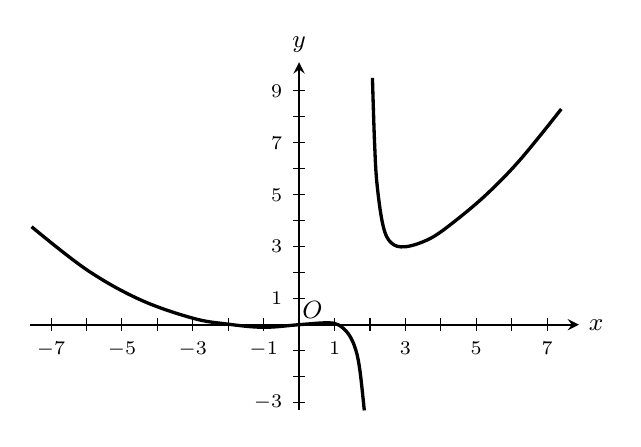
\begin{tikzpicture}[color=black, >=stealth, x=0.45cm, y=0.33cm]
  % Axes: x from about -7.6 to 7.8, y from about -3.3 to 10 (arrows only on the positive ends)
  \draw[->, thick] (-7.6,0) -- (7.9,0);
  \draw[->, thick] (0,-3.3) -- (0,10.1);
  \node[font=\small, anchor=west] at (7.9,0) {$x$};
  \node[font=\small, anchor=south] at (0,10.1) {$y$};
  \node[font=\small, anchor=south west, inner sep=1pt] at (0,0.1) {$O$};
  % Tick marks at every integer
  \foreach \x in {-7,...,-1,1,2,...,7}
    \draw (\x,0.25) -- (\x,-0.25);
  \foreach \y in {-3,-2,-1,1,2,...,9}
    \draw (0.17,\y) -- (-0.17,\y);
  % Tick labels: odd integers only
  \foreach \x in {-7,-5,-3,-1,1,3,5,7}
    \node[font=\scriptsize, anchor=north] at (\x,-0.3) {$\x$};
  \foreach \y in {-3,1,3,5,7,9}
    \node[font=\scriptsize, anchor=east] at (-0.2,\y) {$\y$};
  % Curves, traced from the image (no asymptote line is drawn in the original)
  \begin{scope}
    \clip (-7.6,-3.3) rectangle (7.6,9.6);
    % Left branch: decreasing toward the x-axis, hugs it near x = -2 to 1
    % (slightly below near x = -1, through O, slightly above near x = 0.8),
    % then drops steeply off the bottom just left of x = 2
    \draw[line width=1.2pt] plot[smooth, tension=0.6] coordinates {
      (-7.55,3.77) (-6,2.12) (-4.5,0.97) (-3,0.25) (-2,0.02) (-1,-0.1)
      (0,0) (0.75,0.07) (1.1,0) (1.4,-0.37) (1.6,-0.97) (1.72,-1.8)
      (1.84,-3.3)};
    % Right branch: comes down steeply just right of x = 2, minimum at (3, 3),
    % then rises to about (7.4, 8.3)
    \draw[line width=1.2pt] plot[smooth, tension=0.6] coordinates {
      (2.07,9.5) (2.13,7) (2.2,5.4) (2.37,3.81) (2.6,3.15) (3,3) (3.66,3.29)
      (4.3,3.88) (5.27,4.99) (6.24,6.35) (7.4,8.3)};
  \end{scope}
\end{tikzpicture}
\end{document}
